\documentclass[12pt,final]{amsart}%default 10pt
%prepared in AMSLaTeX, under LaTeX2e

\usepackage[total={6.2in,9.1in},top=1.2in,left=1.1in]{geometry}

\usepackage{natbib}

\usepackage{amssymb,alltt,verbatim,xspace,fancyvrb,color,empheq}
\usepackage{palatino}

% check if we are compiling under latex or pdflatex
\ifx\pdftexversion\undefined
  \usepackage[final,dvips]{graphicx}
\else
  \usepackage[final,pdftex]{graphicx}
\fi

% hyperref should be the last package we load
\usepackage[pdftex,
                colorlinks=true,
                plainpages=false, % only if colorlinks=true
                linkcolor=blue,   % only if colorlinks=true
                citecolor=black,   % only if colorlinks=true
                urlcolor=magenta     % only if colorlinks=true
]{hyperref}

\newcommand{\normalspacing}{\renewcommand{\baselinestretch}{1.1}\tiny\normalsize}
\newcommand{\tablespacing}{\renewcommand{\baselinestretch}{1.0}\tiny\normalsize}
\normalspacing

\definecolor{myblue}{rgb}{.8, .8, 1}

\newcommand*\mybluebox[1]{%
\colorbox{myblue}{\hspace{1em}#1\hspace{1em}}}

% math macros
\newcommand\bv{\mathbf{v}}
\newcommand\bV{\mathbf{V}}
\newcommand\bq{\mathbf{q}}

\newcommand\CC{\mathbb{C}}
\newcommand{\DDt}[1]{\ensuremath{\frac{d #1}{d t}}}
\newcommand{\ddt}[1]{\ensuremath{\frac{\partial #1}{\partial t}}}
\newcommand{\ddx}[1]{\ensuremath{\frac{\partial #1}{\partial x}}}
\newcommand{\ddy}[1]{\ensuremath{\frac{\partial #1}{\partial y}}}
\newcommand{\ddxp}[1]{\ensuremath{\frac{\partial #1}{\partial x'}}}
\newcommand{\ddz}[1]{\ensuremath{\frac{\partial #1}{\partial z}}}
\newcommand{\ddxx}[1]{\ensuremath{\frac{\partial^2 #1}{\partial x^2}}}
\newcommand{\ddyy}[1]{\ensuremath{\frac{\partial^2 #1}{\partial y^2}}}
\newcommand{\ddxy}[1]{\ensuremath{\frac{\partial^2 #1}{\partial x \partial y}}}
\newcommand{\ddzz}[1]{\ensuremath{\frac{\partial^2 #1}{\partial z^2}}}
\newcommand{\Div}{\nabla\cdot}
\newcommand\eps{\epsilon}
\newcommand{\grad}{\nabla}
\newcommand{\ihat}{\mathbf{i}}
\newcommand{\ip}[2]{\ensuremath{\left<#1,#2\right>}}
\newcommand{\jhat}{\mathbf{j}}
\newcommand{\khat}{\mathbf{k}}
\newcommand{\nhat}{\mathbf{n}}
\newcommand\lam{\lambda}
\newcommand\lap{\triangle}
\newcommand\Matlab{\textsc{Matlab}\xspace}
\newcommand\RR{\mathbb{R}}
\newcommand\vf{\varphi}

\newcommand{\Wlij}{W^l_{i,j}}
\newcommand{\Wij}{W_{i,j}}
\newcommand{\Plij}{P^l_{i,j}}
\newcommand{\Pij}{P_{i,j}}
\newcommand{\Ylij}{Y^l_{i,j}}
\newcommand{\Yij}{Y_{i,j}}
\newcommand{\upp}[3]{\big<#1\big|_{#3}\,#2\big>}


\title[]{A less-minimal model of subglacial hydrology}

\author[]{Ward van Pelt and Ed Bueler}


\begin{document}
\maketitle
\thispagestyle{empty}

\section{Introduction}

Any reasonable model of the subglacial aquifer (liquid water layer) has at least these two elements: liquid water is conserved and water flows from high to low hydraulic potential  (``head'').  Additionally, physical processes control the geometry of the layer, including the opening of cavities by sliding and the closure of cavities (and channels) by creep.  Additionally, channels open by melting, sediment moves, and so on, but we do not model these here.

We model water pressure by a damped form of the full-cavity formulation.  In the exactly-full cavity formulation the result is an elliptic variational inequality \citep{Schoofetal2012} for pressure that causes the computation of pressure to be nonlocal over each connected component of the hydrological system.  Here we avoid this instantaneous distributed balance by not exactly enforcing the full-cavity condition.


\section{Elements of a subglacial hydrology continuum model}

We consider a layer of water with thickness $W(t,x,y)$.  This thickness is only likely to be meaningful compared to observations, however, if it is regarded as an average over a horizontal scale of tens to thousands of meters.  As the hydrologic system has fine spatial variation which one is unlikely to be able to model, we will attempt only to model spatially-averaged versions of water amount and water pressure.

We assume that water is incompressible so that the thickness of the water layer tells us the mass of water.  Choosing to model subglacial hydrology using a water thickness is not a significant restriction on the physics.

\subsection*{Conservation}  Water is conserved.  In two spatial dimensions this is the equation \citep{Clarke05}
\begin{equation} \label{eq:conserve}
\frac{\partial W}{\partial t} + \Div \bq = \Phi
\end{equation}
where $\bq$ is the vector water flux (units $\text{m}^2\,\text{s}^{-1}$) and $\Phi$ is a source term ($\text{m}\,\text{s}^{-1}$).

The function $W$ is the key evolving quantity in the model because it is conserved.  It must be saved by the model at any stopping and/or restarting point.  Initial values and boundary values for $W$ must be supplied.  And we always assume this thickness is positive:
\begin{equation}
W \ge 0.
\end{equation}

We might separate the water sources between the melt on the lower surface of the glacier and the en- or supra-glacial drainage origin,
  $$\Phi = \rho_w^{-1} \left(m + S\right)$$
where $\rho_w$ is the density of fresh liquid water, $m$ is the rate at which basal melting (refreeze) of ice adds (removes) water, and $S$ is the rate at which surface runoff or englacial drainage adds water.  Note $m$ and $S$ have units $\text{kg}\,\text{m}^{-2}\,\text{s}^{-1}$.

\newcommand{\Nbreen}{Nordenski\"oldbreen\xspace}
For the \Nbreen, Svalbard example below we will take $m=0$ so that only supraglacial input is modeled.

The water flux $\bq$ in equation \eqref{eq:conserve} is related to the gradient of a hydraulic potential $\psi(t,x,y)$ which combines the actual subglacial water pressure $P(t,x,y)$ and the gravitational potential corresponding to top of the layer of water at the location on the bed of the glacier,
\begin{equation} \label{eq:potential}
\psi = P + \rho_w g\, (b+W).
\end{equation}
Here $z=b(x,y)$ is the time-independent bedrock elevation, which we assume is given by time-independent data.

Water flows from high to low hydraulic potential.  The simplest model is for a water sheet \citep{Clarke05}
\begin{equation}  \label{eq:flux}
\bq = - \frac{K \, W}{\rho_w g} \grad \psi
\end{equation}
Here, $\rho_w$ is the water density ($\text{kg}\,\text{m}^{-3}$), $g$ the gravitational acceleration ($\text{m}\,\text{s}^{-2}$) and $K$ is the effective hydraulic conductivity ($\text{m}\,\text{s}^{-1}$).  Notice that the system transmits more water for a given head gradient if either the ability of the subglacial material to conduct water is bigger (i.e.~$K$ is larger) or if the water sheet is thicker ($W$ is larger).

\subsection*{Advection-diffusion form}  Combining \eqref{eq:potential} and \eqref{eq:flux} above we have this expression which identifies a part of the flux as proportional to the gradient of the water thickness:
	$$\bq = - \frac{K\, W}{\rho_w g} \left(\grad P + \rho_w g b\right) - K W \grad W.$$
The flux which is down the gradient of the conserved quantity will act diffusively.  The remaining flux is likely to be dominant.  It is, to our knowledge, not particularly diffusive.  We conceive of it as transport driven by a velocity field which varies in space and time.  We will construct a conservative numerical scheme based on this understand of how the flux is decomposed.

Let
\begin{equation} \label{eq:vexpression}
  \bV = - \frac{K}{\rho_w g} \grad P - K \grad b
\end{equation}
be the velocity field.  Then equations \eqref{eq:potential}, \eqref{eq:flux}, and \eqref{eq:vexpression} combine to this simpler description of the flux,
\begin{equation} \label{eq:qexpression}
  \bq = \bV\, W - K W \grad W.
\end{equation}

Generally the water flow $\bq$ depends significantly on the ice surface slope because the gradient of the overburden pressure follows that slope.  The pressure model below may generate pressure fields with that property, but this is not obvious.  More obviously the flux depends on the bedrock slope because the velocity $\bV$ has such a term.  Because the bedrock elevation comes from rough data in practice, this part of the velocity $\bV$ will not be very smooth.  The part of the flux from the pressure gradient may not be very smooth either, depending on the solution of the pressure model below.

In any case, from equations \eqref{eq:conserve} and \eqref{eq:qexpression} we derive an advection-diffusion equation \citep{HundsdorferVerwer2010,MortonMayers} for the evolution of the water layer thickness:
\begin{equation} \label{eq:adeqn}
  \frac{\partial W}{\partial t} + \Div\left(\bV\, W\right) = \Div \left(K W \grad W\right) + \Phi.
\end{equation}
As we will see, the significance of this form is that there are numerical differences in how the advection term $\Div\left(\bV\, W\right)$ is handled relative to the diffusion term $\Div \left(K W \grad W\right)$.

\subsection*{Capacity of the linked-cavity system}  First recall that the ice is a fluid which has a pressure field of its own, with basal value $P_o$, the \emph{overburden pressure}.  We make the shallow approximation that the ice pressure is hydrostatic \citep{GreveBlatter2009}:
\begin{equation} \label{eq:hydrostatic}
  P_o = \rho_i g H = \rho_i g (h-b).
\end{equation}
Here $\rho_i$ is the density of ice ($\text{kg}\,\text{m}^{-3}$), $H$ is the ice thickness (m), and $h$ is the ice upper surface elevation (m).  Now let
\begin{equation}
N = P_o - P\label{eq:effective}
\end{equation}
be the effective pressure.  The effective pressure is high if the subglacial water is unpressurized and low in the high pressure water case.  The effective pressure is a measure of much of the ice load is carried by the mineral (till or bedrock) base.

The evolution of the capacity thickness $Y$ (m) of a linked-cavity system is described as the sum of opening by cavitation and closure by creep:
\begin{equation}
\frac{\partial Y}{\partial t} = c_1 |\bv_b| \min\left\{0,W_r - Y\right\} - c_2 A |N|^3 Y, \label{eq:capacity}
\end{equation}
where $W_r$ is a maximum roughness scale of the basal topography, $\bv_b$ is the ice basal velocity (i.e.~sliding velocity), $A$ is the ice softness, and $c_1,c_2$ are constants to be fit by data (see below).  We have used Glen exponent $n=3$ for concreteness.

Equation \eqref{eq:capacity} describes the evolution of the upper (ice) surface of the subglacial cavity.  The first term in \eqref{eq:capacity}, the cavitation term, is always nonnegative (i.e.~causes opening), and it is only positive where the capacity is less than the roughness scale, namely $Y<W_r$.  The other term describing creep is sensitive to the difference of ice and water pressure, but ice creep is relatively slow.  There are presumably-strong stresses (pressures) within the liquid water associated to keeping the cavity full because liquid water is an incompressible fluid with low viscosity.

For example, if the cavity is locally larger than local water sources can easily fill then the pressure should be locally lower, and this should cause inflow into this local area, assuming water is available in connected cavities.  Conversely, if local water sources exceed capacity then the pressure field should force water out of the local area.  Only if there is insufficient connection to neighboring capacity should the extreme cases occur, wherein a vapor (e.g. air) layer forms in the cavity, or the ice is forced upward by a negative effective pressure, respectively.


\section{Closures to determine pressure}

At this point we do not know how to compute pressure $P$.  The apparent state variables of the model so far are $W$,$Y$,$P$.  For a fixed ice geometry and ice velocity, the above equations can be written as two partial differential equations in these three variables.   (Of course there are several additional data functions and parameters.)  Two equations are not enough to determine these variables, however.  A closure for the pressure is needed.

\subsection*{Full-cavity closure}  Requiring the aquifer to be full at all locations and times is a closure:
\begin{equation}
W = Y.\label{eq:strongclosure}
\end{equation}
The consequences of this ``strong'' closure are explored by \cite{Schoofetal2012}, in a broader context.  Equation \eqref{eq:strongclosure} allows us to eliminate $Y$, but we can also use the time-derivative of the strong closure, namely the equality $\partial W/\partial t = \partial Y/\partial t$.  From equations \eqref{eq:conserve}, \eqref{eq:potential}, \eqref{eq:flux}, and \eqref{eq:capacity}, and using $\partial W/\partial t = \partial Y/\partial t$ to eliminate the time derivatives, we get this equation relating $P$ and $W$:
\begin{equation}
\Div \left(\frac{K\,W}{\rho_w g} \grad \left(P + \rho_w g (b+W)\right) \right) + \Phi = c_1 |\bv_b| \min\left\{0,W_r - W\right\} - c_2 A |P_o - P|^3 W.\label{eq:ellipticpressure}
\end{equation}
Equation \eqref{eq:ellipticpressure} is essentially the same as equation (2.12) in \citep{Schoofetal2012}.

Though we will not solve \eqref{eq:ellipticpressure} directly, this equation is very significant to the understanding of the structure of the mathematical model which we will eventually solve.  Specifically, in a region where the water thickness field $W$ is positive, \eqref{eq:ellipticpressure} is an elliptic PDE for the unknown pressure $P$.  Because $P$ is nonnegative, and because the condition $P>P_o$ is presumed to cause the ice to lift quickly and thus lower the pressure back to overburden $P=P_o$, the pressure solution is subject to inequalities
\begin{equation}
0 \le P \le P_o. \label{eq:bounds}
\end{equation}
The mathematical subproblem encompassing \eqref{eq:ellipticpressure}, constraints \eqref{eq:bounds}, and adequate pressure boundary conditions is all together an elliptic variational inequality \citep{KinderlehrerStampacchia}.  This mathematical model is explored by \cite{Schoofetal2012}.  The numerical analysis of such problems can be addressed with a finite element approach \citep{SchoofStream,JouvetBueler2012}.

However, the goal of the current work is the initial selection of a usable subglacial hydrology model which can be coupled to ice dynamics.  We need to determine parameters from observations.  These goals suggest the need for rapid implementation.  Therefore, in these notes, we seek an easily-implemented finite difference model which does not require the solution of an elliptic problem at each time step.

\subsection*{Nearly-full-cavity closure}  Therefore we propose, as one possible alternative, to replace rigid constraint \eqref{eq:strongclosure}, namely $0 = Y - W$, with a damped version.  Choose a characteristic time scale $\tau$ which should be short (hours to months) compared to ice flow change time scales (months to centuries).  Then consider this equation
\begin{equation}
- \tau \frac{\partial Y}{\partial t} = Y - W. \label{eq:dampedclosure}
\end{equation}
As $\tau \to 0$ this equation recovers the full-cavity closure $Y=W$.  It says that if the notional cavity upper surface ($Y$) is locally above the water level ($Y>W$) then it should lower ($\partial Y/\partial t < 0$), and, vice versa, if the notional cavity upper surface is locally below the water ($Y<W$) then the cavity top should rise ($\partial Y/\partial t > 0$).   Said a different way, equation \eqref{eq:dampedclosure} represents a penalty method for enforcing constraint \eqref{eq:strongclosure}.  Equation \eqref{eq:dampedclosure} requires us to keep the separate state variable $Y$ in a time-dependent way.  It does not allow us to eliminate $Y$.

On the other hand, equation \eqref{eq:dampedclosure} allows us to express pressure in terms of the geometric state variables $W$ and $Y$, as follows.  Solve \eqref{eq:capacity} for $N$, thus $P$, and substitute the expression for $\partial Y/\partial t$ from \eqref{eq:dampedclosure}:
\begin{equation}
P = P_o - \left(\frac{\tau^{-1} (Y-W) + c_1 |\bv_b| \min\left\{0,W_r - Y\right\}}{c_2 A Y}\right)^{1/3}.  \label{eq:pressurenormal}
\end{equation}

The above expression for $P$ applies only in certain ``normal'' cases, however.  In particular it assumes positive effective pressure ($N\ge 0$).  Furthermore we must address how the bounds \eqref{eq:bounds} are maintained.  Note that the denominator of the fraction in \eqref{eq:pressurenormal} is always positive but the denominator can change sign.  Let $\mathcal{Z} = \tau^{-1} (Y-W) + c_1 |\bv_b| \min\left\{0,W_r - Y\right\}$,  the numerator appearing in Equation \eqref{eq:pressurenormal}.  We have the following conditional scheme for pressure:
\begin{equation}
P = \begin{cases}
0, & \mathcal{Z} \ge c_2 A Y P_o^3\,\, (\ge 0) , \\
P_o, & \mathcal{Z} \le 0, \\
P_o - \mathcal{Z}^{1/3} (c_2 A Y)^{-1/3}, & \text{all other cases}.
\end{cases} \label{eq:pressureWY}
\end{equation}
The last ``normal pressure'' case occurs exactly when the given formula computes a pressure satisfying \eqref{eq:bounds}.  As a result of this scheme we have a function which computes pressure in terms of $Y,W$, namely $P = f(Y,W)$.  Of course $f$ is also a function of model parameters (i.e.~$W_r,c_1,c_2,\dots$) and of ice flow model variables (i.e.~$P_o,|\bv_b|$).

The above equations have now yielded a solvable mathematical model, but the reader deserves a clarified version.  We can apply the several definitions at each time step, starting with the geometric data $h,b$ and the current values of the state variables $W,Y$ and computing $P_o$, $\mathcal{Z}$, $P$, and $\bV$ in turn.  Then the time step itself is for these two evolution equations, which are equations \eqref{eq:adeqn} and \eqref{eq:dampedclosure}, respectively,
\begin{align}
\frac{\partial W}{\partial t} + \Div\left(\bV\, W\right) &= \Div \left(K W \grad W\right) + \Phi, \label{eq:AGAINadeqn} \\
\frac{\partial Y}{\partial t} &= \frac{Y - W}{-\tau}. \label{eq:AGAINdampedclosure}
\end{align}

\subsection*{Alternative nearly-full closure}  As already noted, we observe that an important consequence of the full-cavity identity $Y=W$ (i.e.~equation \eqref{eq:strongclosure}) is the elliptic PDE \eqref{eq:ellipticpressure}.  This PDE describes how the pressures of different areas of the aquifer are related to each other at each instant.  However, the model in the previous subsection, equations \eqref{eq:AGAINadeqn}--\eqref{eq:AGAINdampedclosure}, does not obviously support a damped version of instantaneous relation \eqref{eq:ellipticpressure}.  In this subsection we try again, using both \eqref{eq:strongclosure} and a different nearly-full version of it, to build a model which contains a damped version of \eqref{eq:ellipticpressure}.

Let $E_0>0$ be a fixed, small vertical distance which is a fraction of the typical aquifer thickness.  We approximate the time derivative of $Y=W$, the identity $\partial W/\partial t = \partial Y/\partial t$, by this new damped version:
\begin{equation}
\frac{E_0}{P_o} \frac{\partial P}{\partial t} =  \frac{\partial W}{\partial t}  - \frac{\partial Y}{\partial t}.\label{eq:dampeddstrong}
\end{equation}
Note that the units do match, so that the equation has units $\text{m}\,\text{s}^{-1}$.  As with the previous nearly-full relation \eqref{eq:dampedclosure}, equation \eqref{eq:dampeddstrong} represents a penalty method for enforcing constraint \eqref{eq:strongclosure}.  The $E_0\to 0$ (singular) limit of equation \eqref{eq:dampeddstrong} recovers $\partial W/\partial t = \partial Y/\partial t$, and thus elliptic PDE \eqref{eq:ellipticpressure} also.

Note that $E_0/P_o$ is a positive in any area where there is ice.  Therefore, in equation \eqref{eq:dampeddstrong}, $P$ increases when $W$ is growing faster than $Y$ (e.g.~if the aquifer is being forced open by water).  Conversely, $P$ decreases when $Y$ is growing faster than $W$ (e.g.~if cavitation is trying to open space for water but water is being supplied slower than that).

Equation \eqref{eq:dampeddstrong} implies a replacement for elliptic equation.  Specifically, by using the expressions from \eqref{eq:conserve}, \eqref{eq:potential}, and \eqref{eq:flux} for $\partial W/\partial t$, and by using the expression from \eqref{eq:capacity} for $\partial Y/\partial t$, and also using the identity $Y=W$ to eliminate $Y$, we get this equation:
\begin{align}
\frac{E_0}{P_o} \frac{\partial P}{\partial t} &= \Div \left(\frac{K\,W}{\rho_w g} \grad (P+\rho_w g (b+W))\right) - c_1 |\bv_b| \min\left\{0,W_r - W\right\} \label{eq:diffusionpressure} \\
  &\qquad\qquad + c_2 A |P_o - P|^3 W  + \Phi. \notag
\end{align}

In any region where $W>0$, equation \eqref{eq:diffusionpressure} is a diffusion, a parabolic equation for $P$.  In fact, at this stage we have a new mathematical model, consisting of conservation equation \eqref{eq:adeqn} for evolution of $W$, equation \eqref{eq:diffusionpressure} for evolution of pressure $P$, and the bounds on $W$ and $P$.  Again let $c_0 = K / \rho_w g$.  Here is our proposed mathematical model:
\begin{empheq}[box=\mybluebox]{align}
0 &\le W, \label{eq:ALTWbound} \\
0 &\le P \le P_o, \label{eq:ALTbounds} \\
\bV &= - c_0 \grad P - K \grad b, \label{eq:ALTvexpression} \\
\psi &= P + \rho_w g (b + W), \label{eq:ALTpotential} \\
\frac{\partial W}{\partial t} + \Div\left(\bV\, W\right) &= \Div \left(K W \grad W\right) + \Phi \label{eq:ALTadeqn} \\
\frac{E_0}{P_o} \frac{\partial P}{\partial t} &= \Div \left(c_0\,W\, \grad \psi \right) + c_2 A |P_o - P|^3 W \label{eq:ALTdiffusionpressure} \\
  &\qquad - c_1 |\bv_b| \min\left\{0,W_r - W\right\} + \Phi. \notag
\end{empheq}


\subsection*{On the symbols}  The above equations \eqref{eq:ALTWbound}--\eqref{eq:ALTdiffusionpressure} relate four classes of symbols, as summarized in the following table:

\begin{table}[h]
\begin{tabular}{r|c}
class & symbols \\ \hline
\emph{parameters (scalar)} & $g$, $\rho_i$, $\rho_w$, $A$, $K$, $W_r$, $c_0$, $c_1$, $c_2$, $\tau$ \\
\emph{data functions} & $\Phi$, $b$, $h$, $|\bv_b|$ \\
\emph{derived functions} & $\bV$, $\psi$ \\
\emph{state functions} & $W$, $P$
\end{tabular}
\end{table}

\noindent The parameters are constant (i.e.~time- and space-independent).  Default values must be chosen for these parameters, even though the informed model user will seek to change these values and explore the parameter space.  The data functions are, essentially, supplied by the rest of the ice sheet model.

The state and derived functions evolve according to the mathematical model in this work, but only the state functions $W,P$ must be provided with initial values, and saved for restarting the model.



\section{Numerical scheme}

\subsection*{Numerical scheme for conservation equation \eqref{eq:adeqn}}  Equation \eqref{eq:adeqn} will be discretized in this section by an explicit conservative first-order upwind method for the advection part and an explicit centered, second-order scheme for the nonlinear diffusion part.

Because this is an explicit scheme, we consider stable time steps immediately.  It turns out that the time step restriction for the advective part, i.e.~the CFL condition on the upwind scheme, is much more restrictive than the time-step restriction for the diffusion in \eqref{eq:adeqn}.  In fact, in the Appendix it is shown that the time step must satisfy
\begin{equation}
\Delta t_{\text{CFL}} \left(\frac{\max |\alpha|}{\Delta x} + \frac{\max |\beta|}{\Delta y}\right) \le \frac{1}{2} \label{eq:dtCFL}
\end{equation}
where $V=(\alpha,\beta)$ is the advecting velocity, for the upwind part of the scheme to maintain stability.  The time step must also satisfy
\begin{equation}
\Delta t_W\, (2 K \max W) \left(\frac{1}{\Delta x^2} + \frac{1}{\Delta y^2}\right) \le \frac{1}{2} \label{eq:dtDIFFW}
\end{equation}
for the diffusion scheme to be stable.

To give some practical values for these time step restrictions, we are interested in grids of size $\Delta x = \Delta y = 500$ m.  The maximum speed $|\bV|$ is about $10^5$ m/a in trial runs of the model, so $\max |\alpha| = \max |\beta| \approx 0.002$ m/s.  We take $K=10^{-2}$ m/s and $\max W=1$ m as representative values.  In that case the advective restriction \eqref{eq:dtCFL} gives about $\Delta t_{\text{CFL}} \le 0.001$ year while the diffusive restriction from \eqref{eq:dtDIFFW} is about $\Delta t_W \le 0.1$ year.  Thus, unless velocities are unusually slow and deep lakes develop (so that $KW$ is large), we should not worry so much about the diffusive time scale.  The problem is primarily an advection.

To set notation to actually state the scheme, suppose our rectangular computational domain has $M_x \times M_y$ gridpoints $(x_i,y_j)$ with uniform spacing $\Delta x,\Delta y$.  Let $\Wlij \approx W(t_l,x_i,y_j)$ and $\Ylij \approx Y(t_l,x_i,y_j)$ be the approximations of the continuum solution at the grid points.

To explain the upwind method for \eqref{eq:adeqn}, consider the model equation
\begin{equation} \label{eq:modeladvect}
u_t + (v(x) u)_x = 0
\end{equation}
for some quantity $u(t,x)$ transported by a flux $q = v(x) u$.  A ``donor cell'' upwind scheme can be described as a finite volume scheme \citep{LeVeque} wherein a grid point $x_j$ is the center of a cell.  We consider the flux at the cell interfaces $x_{j-1/2}$ and $x_{j+1/2}$.  We decide which spatial finite difference to compute based on the sign of the velocity $v(x)$ at these interfaces.

The scheme is easier to display if we define the following upwind notation,
\newcommand{\up}[2]{\big<#1\big|\,#2\big>}
	$$\up{v}{U_j} := v \begin{Bmatrix} U_j, & v \ge 0 \\ U_{j+1}, & v < 0 \end{Bmatrix}.$$
For the model equation \eqref{eq:modeladvect} on a space-time grid $(t_l,x_j)$ we set
\begin{equation}\label{eq:modelfdadvect}
\frac{U_j^{l+1} - U_j^l}{\Delta t} + \frac{\up{v_+}{U_j^l} - \up{v_-}{U_{j-1}^l}}{\Delta x} = 0
\end{equation}
where $v_+ = v(x_{j+1/2})$ and $v_-=v(x_{j-1/2})$.

\begin{figure}[ht]
\centering
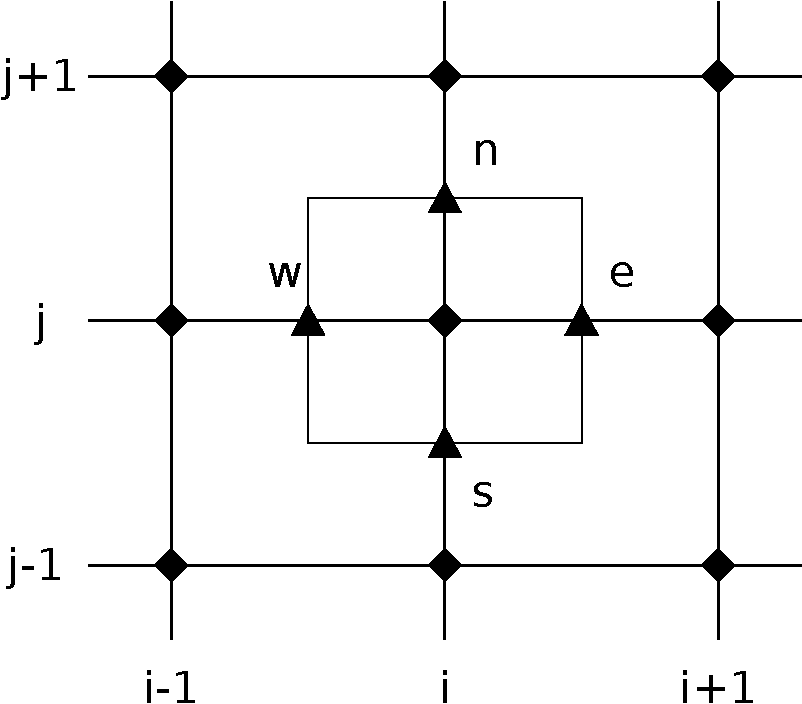
\includegraphics[width=2.0in,keepaspectratio=true]{figs/diffstencil}
\bigskip
\caption{The numerical scheme for Equation \eqref{eq:adeqn} is a finite volume scheme for the grid-centered cell (dashed line).  The velocity and diffusivities are evaluated at the staggered grid locations (triangles).  The state functions $W,Y$ are needed at the regular grid points (diamonds).}
\label{fig:stencil}
\end{figure}

Now we can state our scheme for equation \eqref{eq:adeqn}, starting with the coefficients.  Suppose the velocity has components $\bV = (\alpha,\beta)$ and recall that $\Div \left(\bV W\right) = (\alpha W)_x + (\beta W)_y$.  We will compute velocity components at staggered (cell-face-centered) points, shown with triangle markers in Figure \ref{fig:stencil}.  We compute these values based on centered finite difference approximations of Equation \eqref{eq:vexpression}.

Let $c_0=K/(\rho_w g)$, a derived parameter used for convenience, which allows us to write a simplest description of the velocity:  $\bV = - c_0 \grad P - K \grad b$.  We use ``compass'' notation for the components:
\begin{align*}
\alpha_e &= \alpha_{i+1/2,j} = - c_0 \frac{P_{i+1,j}-P_{i,j}}{\Delta x} - K \frac{b_{i+1,j}-b_{i,j}}{\Delta x}, \\
\alpha_w &= \alpha_{i-1/2,j} = - c_0 \frac{P_{i,j}-P_{i-1,j}}{\Delta x} - K \frac{b_{i,j}-b_{i-1,j}}{\Delta x}, \\
\beta_n  &= \beta_{i,j+1/2} = - c_0 \frac{P_{i,j+1}-P_{i,j}}{\Delta y} - K \frac{b_{i,j+1}-b_{i,j}}{\Delta y}, \\
\beta_s  &= \beta_{i,j-1/2} = - c_0 \frac{P_{i,j}-P_{i,j-1}}{\Delta y} - K \frac{b_{i,j}-b_{i,j-1}}{\Delta y}.
\end{align*}

Similarly for the diffusive term, the staggered-grid values of the current water thicknesses are computed by averaging:
\begin{align*}
W_e &= (W_{i,j}^l + W_{i+1,j}^l)/2, & W_w &= (W_{i-1,j}^l + W_{i,j}^l)/2, \\
W_n &= (W_{i,j}^l + W_{i,j+1}^l)/2, & W_s &= (W_{i,j-1}^l + W_{i,j}^l)/2.
\end{align*}

We apply the conservative upwind scheme in each variable, indicating the active index (either $i$ or $j$) in our upwind notation:
\begin{align}
 &\frac{W_{i,j}^{l+1} - \Wlij}{\Delta t} + \frac{\upp{\alpha_e}{\Wlij}{i} - \upp{\alpha_w}{W_{i-1,j}^l}{i}}{\Delta x} + \frac{\upp{\beta_n}{\Wlij}{j} - \upp{\beta_s}{W_{i,j-1}^l}{j}}{\Delta y}  \label{eq:Wfd} \\
      &\qquad = K \bigg[\frac{W_e \left(W_{i+1,j}^l - \Wlij\right) - W_w \left(\Wlij - W_{i-1,j}^l\right)}{\Delta x^2}  \notag \\
      &\qquad\qquad\qquad + \frac{W_n \left(W_{i,j+1}^l - \Wlij\right) - W_s \left(\Wlij - W_{i,j-1}^l\right)}{\Delta y^2}\bigg] + \Phi_{ij}. \notag
\end{align}
Because of the first-order upwinding this scheme has $O(\Delta t^1 + \Delta x^1 + \Delta y^1)$ truncation error.

Because of the positivity proven in the appendix for this scheme, if $\Phi\ge 0$ then the lower bound $W\ge 0$ is true for the updated values at the new time $t_{l+1}$.  However, because refreeze is possible, generally we must enforce $W\ge 0$ on the updated values.  If $W_{i,j}^{l+1}<0$ at the end of a step we reset $W_{i,j}^{l+1}=0$.  The amount of mass created by this step should be accounted for.  As the temporal grid is refined, the conservation error should decrease.


\subsection*{Numerical scheme for nearly-full equation \eqref{eq:AGAINdampedclosure}}    Equation \eqref{eq:AGAINdampedclosure} will be discretized by a semi-implicit first-order Euler method (implicit for $Y$ and explicit for $W$).  Here we are not troubled by spatial derivatives.  The scheme we propose depends on first having computed the updated water thickness $W_{i,j}^{l+1}$ from \eqref{eq:Wfd}.  The scheme we propose is first-order backward Euler \citep{BurdenFaires} for the time-dependent ODE \eqref{eq:AGAINdampedclosure}, thus
\begin{equation}
\frac{Y_{i,j}^{l+1} - Y_{i,j}^{l}}{\Delta t} = \frac{Y_{i,j}^{l+1} - W_{i,j}^{l+1}}{- \tau}. \label{eq:Yfd}
\end{equation}
This proposed scheme is a maximally-stable first draft numerical scheme.  It can be rewritten as a direct calculation of the updated value,
   $$Y_{i,j}^{l+1} = \frac{1}{1 + (\Delta t/\tau)}\, Y_{i,j}^{l} + \frac{1}{1 + (\tau / \Delta t)}\, W_{i,j}^{l+1}.$$
It follows that for \emph{any} time step $\Delta t$ we compute $Y_{i,j}^{l+1}$ as a linear combination of $Y_{i,j}^{l}$ and $W_{i,j}^{l+1}$ with coefficients which are each positive and each less than one, and which add to one.  Thus the scheme is unconditionally stable.


\subsection*{Numerical scheme for alternative nearly-full equation \eqref{eq:ALTdiffusionpressure}}   Equation \eqref{eq:ALTdiffusionpressure} is, like equation \eqref{eq:adeqn}, a diffusion.  This time there are additional ``reaction'' terms, but no dominating advection terms.  Again it will be discretized by an explicit centered, second-order scheme for the nonlinear diffusion part.  And again, because this is an explicit scheme, we consider stable time steps immediately.

The time step restriction is comparable to \eqref{eq:dtDIFFW}, though the proof in the appendix does not suffice to \emph{prove} stability under this condition because of the additional reaction terms.  Noting that $P_o=\rho_i g H$,
\begin{equation}
\Delta t_P\, \left(\frac{2 K \rho_i \max H \max W}{\rho_w E_0}\right) \left(\frac{1}{\Delta x^2} + \frac{1}{\Delta y^2}\right) \le \frac{1}{2} \label{eq:dtDIFFP}
\end{equation}
The resulting time step is a certain fraction of the time step from \eqref{eq:dtDIFFW},
\begin{equation}
\Delta t_P = \frac{\rho_w E_0}{\rho_i \max H}\, \Delta t_W.
\end{equation}

With the estimates $\rho_w/\rho_i \approx 1$, $E_0\approx 1$ m, and $\max H \approx 1000$ m we have a pressure-update time step $\Delta t_P$ which is about 1000 times smaller than the time step $\Delta t_W$.  With these values and the previous ones identified earlier (i.e.~$\Delta x = \Delta y = 500$ m, $\max |\bV|=10^5$ m/a, $K=10^{-2}$ m/s and $\max W=1$ m) we get
\begin{align*}
  \Delta t_{\text{CFL}} &\le 0.001  \text{ year} &&\text{ from \eqref{eq:dtCFL}}, \\
  \Delta t_W            &\le 0.1    \text{ year} &&\text{ from \eqref{eq:dtDIFFW}}, \\
  \Delta t_P            &\le 0.0001 \text{ year} &&\text{ from \eqref{eq:dtDIFFP}.}
\end{align*}
Thus the numerical scheme for pressure diffusion \eqref{eq:ALTdiffusionpressure}, given below, has the shortest time step but it might only be about 10 times shorter than the essentially-obligatory CFL restriction for the advection.  Furthermore, the precise size of the stable time step $\Delta t_P$ scales inversely with the adjustable small thickness $E_0$; by choosing $E_0$ larger we can make the time step restriction on $\Delta t_P$ less severe.

The scheme we use for \eqref{eq:ALTdiffusionpressure} is similar to \eqref{eq:Wfd} for \eqref{eq:adeqn}:
\begin{align}
\frac{E_0}{P_o} \frac{P_{i,j}^{l+1} - \Plij}{\Delta t} &= c_0 \bigg[\frac{W_e \left(\psi_{i+1,j}^l - \psi_{i,j}^l\right) - W_w \left(\psi_{i,j}^l - \psi_{i-1,j}^l\right)}{\Delta x^2}  \label{eq:Pfd} \\
      &\qquad\qquad + \frac{W_n \left(\psi_{i,j+1}^l - \psi_{i,j}^l\right) - W_s \left(\psi_{i,j}^l - \psi_{i,j-1}^l\right)}{\Delta y^2}\bigg] \notag \\
      &\qquad + c_2 A \left|\rho_i g H_{i,j} - \Plij\right|^3 W - c_1 |\bv_b|_{i,j} \min\left\{0,W_r - \Wlij\right\} + \Phi_{i,j}. \notag
\end{align}
At the start of each step we compute the current values of the hydraulic potential,
	$$\psi_{i,j}^l = \Plij + \rho_w g(b_{i,j} + \Wlij).$$

Generally there is no expectation that this pressure update will preserve our bounds \eqref{eq:ALTbounds}, namely $0\le P \le P_o$.  Thus, at the end of each pressure-update time step we must explicitly \emph{project} to put the pressure $P_{i,j}^{l+1}$ back into this correct range.  Note that pressure is not a conserved quantity, so this projection step does not have accounting issues like that for the update to $W$.


%\clearpage \newpage
\small
\bibliography{ice_bib}  % generally requires link to pism/doc/ice_bib.bib
\bibliographystyle{agu}


%\clearpage \newpage
\small
\appendix

\section{Positivity and stability of the numerical scheme}

Explicit numerical scheme \eqref{eq:Wfd} for the model PDE \eqref{eq:adeqn} is sufficiently simple so that we can analyze its properties.  The scheme is conditionally stable with conditions we give below.  We also note that the scheme is positivity-preserving: if the water input $\Phi$ is nonnegative and the discrete water thicknesses $\Wlij$ are also nonnegative at step $t_l$ then, under the stability conditions, the updated values $W_{i,j}^{l+1}$ are also nonnegative.  In this appendix we sketch a maximum principle argument \citep{MortonMayers} which shows both stability and the positivity-preserving property.

Let $\nu_x = \Delta t/\Delta x$, $\nu_y = \Delta t/\Delta y$, $\mu_x = K \Delta t / (\Delta x)^2$, and $\mu_y = K \Delta t / (\Delta y)^2$.  We consider only the case where all of the discrete velocities at the middle of the cell edges are nonnegative: $\alpha_e\ge 0$, $\alpha_w\ge 0$, $\beta_n\ge 0$, $\beta_s\ge 0$.  The many other cases, where these velocity components have various signs, can be handled by similar special-case arguments like the present one, and these other cases are left as a standard exercise for the reader \citep{MortonMayers}.

We rewrite \eqref{eq:Wfd} as a computation of the next value $W_{i,j}^{l+1}$, and collect terms:
\begin{align*}
 W_{i,j}^{l+1} &= \Wlij - \nu_x \left(\alpha_e \Wlij - \alpha_w W_{i-1,j}^l\right) - \nu_y \left(\beta_n \Wlij - \beta_s W_{i,j-1}^l\right)  \\
      &\qquad + \mu_x \left[W_e \left(W_{i+1,j}^l - \Wlij\right) - W_w \left(\Wlij - W_{i-1,j}^l\right)\right]  \\
      &\qquad + \mu_y \left[W_n \left(W_{i,j+1}^l - \Wlij\right) - W_s \left(\Wlij - W_{i,j-1}^l\right)\right] + \Delta t \Phi_{ij} \\
      &= (\nu_x \alpha_w + \mu_x W_w) W_{i-1,j}^l + (\mu_x W_e) W_{i+1,j}^l + (\nu_y \beta_s + \mu_y W_s) W_{i,j-1}^l + (\mu_y W_n) W_{i,j+1}^l \\
      &\qquad + \Big[1 - \nu_x \alpha_e - \nu_y \beta_n - \mu_x (W_e + W_w) - \mu_y (W_n + W_s)\Big] \Wlij + \Delta t \Phi_{ij}.
\end{align*}
The new value is a linear combination of the old values, plus a source term:
\begin{equation}
W_{i,j}^{l+1} = A W_{i-1,j}^l + B W_{i+1,j}^l + C W_{i,j-1}^l + D W_{i,j+1}^l + E \Wlij + \Delta t \Phi_{ij}. \label{eq:lincomb}
\end{equation}

Because of our assumption about nonnegative velocities, and assuming $\Wlij \ge 0$ for all $i,j$, coefficients $A,B,C,D$ are all nonnegative, and only $E$ could be negative, depending on the time step.  Thus we can state a sufficient condition based on an equal split between advective and diffusive parts.

Let us assume a CFL-type time step restriction for the advection term in  \eqref{eq:adeqn}:
\begin{equation}
\nu_x \alpha_e + \nu_y \beta_n = \Delta t \left(\frac{\alpha_e}{\Delta x} + \frac{\beta_n}{\Delta y}\right) \le \frac{1}{2}. \label{eq:adstabcond}
\end{equation}
Because we also handle the diffusion term in \eqref{eq:adeqn} explicitly, we have second time-step restriction:
\begin{equation}
\mu_x (W_e + W_w) + \mu_y (W_n + W_s) = \Delta t \left(\frac{K(W_e + W_w)}{\Delta x^2} + \frac{K(W_n + W_s)}{\Delta y^2}\right) \le \frac{1}{2}. \label{eq:diffstabcond}
\end{equation}
The right-hand sides of these inequalities are each $1/2$, but of course $1-(1/2)-(1/2)=0$.  In other words the coefficient $E$ in \eqref{eq:lincomb} is nonnegative:
	$$E = 1 - \nu_x \alpha_e - \nu_y \beta_n - \mu_x (W_e + W_w) - \mu_y (W_n + W_s) \ge 0.$$

Though the argument can only be made fully rigorous by handling all upwind cases (not shown), we see that all coefficients in linear combination \eqref{eq:lincomb} are nonnegative.  Furthermore they all add to one.  It follows \citep{MortonMayers} that scheme \eqref{eq:Wfd} is positivity-preserving when $\Phi\ge 0$, and it is stable under the stability conditions \eqref{eq:adstabcond} and \eqref{eq:diffstabcond}.

\end{document}
